\subsection{Ergebnisse der Testmethode}
\label{subsec:ergebnisse-der-testmethoden}
In der folgenden Tabelle \ref{tab: Tabelle der Testergebnisse} werden die Ergebnisse grob dargestellt.
Die Erläuterung der aufgetretenen Mängel wird im Folgenden genauer beschrieben und erste Lösungsansätze werden genannt.


\begin{table}[H]
    \centering

    \setlength{\tabcolsep}{3pt} % reduziert Spaltenabstand
    \resizebox{\textwidth}{!}{ % skaliert Tabelle auf Textbreite
    \begin{tabular}{|c|c|c|c|c|c|c|}
        \hline
        \textbf{DUT-Type} &
        \textbf{Ergebnisse des Berichtes} &
        \textbf{Einlesen} &
        \textbf{Datenbankeinträge vorhanden} &
        \textbf{Tabelleneintrag vorhanden} &
        \textbf{Graphen vorhanden} &
        \textbf{Aufgetretene Fehler} \\
        \hline
        \rowcolor{green!15}
        124 & Erfolgreich & Erfolgreich & Vorhanden und korrekt & Vorhanden und korrekt & Vorhanden und korrekt & Keine \\
        \hline
        \rowcolor{green!15}
        124 & Fehler & Erfolgreich & Vorhanden und korrekt & Vorhanden und korrekt & Erwartete Werte vorhanden & Keine \\
        \hline
        \rowcolor{yellow!15}
        119 & Erfolgreich & Erfolgreich & Vorhanden und korrekt & Vorhanden und korrekt & Flowrate-Graph fehlt & Anderer Name für Flowrate \\
        \hline
        \rowcolor{green!15}
        119 & Fehler & Erfolgreich & Vorhanden und korrekt & Vorhanden und korrekt & Keine vorhanden (erwartet) & Keine \\
        \hline
        \rowcolor{red!15}
        118 & Erfolgreich & Fehler & Keine vorhanden & Keine vorhanden & Keine vorhanden & Fehler durch fehlende Seriennummern \\
        \hline
        \rowcolor{red!15}
        118 & Fehler & Fehler & Keine vorhanden & Keine vorhanden & Keine vorhanden & Fehler durch fehlende Seriennummern \\
        \hline
        \rowcolor{yellow!15}
        114 & Erfolgreich & Erfolgreich & Vorhanden und korrekt & Vorhanden und korrekt & Flowrate-Graph fehlt & Anderer Name für Flowrate \\
        \hline
        \rowcolor{yellow!15}
        114 & Fehler & Erfolgreich & Vorhanden und korrekt & Vorhanden und korrekt & Flowrate-Graph fehlt & Anderer Name für Flowrate \\
        \hline
        \rowcolor{yellow!15}
        112 & Erfolgreich & Erfolgreich & Vorhanden und korrekt & Vorhanden und korrekt & Flowrate-Graph fehlt & Anderer Name für Flowrate \\
        \hline
        \rowcolor{yellow!15}
        112 & Fehler & Erfolgreich & Vorhanden und korrekt & Vorhanden und korrekt & Flowrate Graph-fehlt & Anderer Name für Flowrate \\
        \hline
        \rowcolor{yellow!15}
        113 & Erfolgreich & Erfolgreich & Vorhanden und korrekt & Vorhanden und korrekt & Flowrate-Graph fehlt & Anderer Name für Flowrate \\
        \hline
        \rowcolor{yellow!15}
        113 & Fehler & Erfolgreich & Vorhanden und korrekt & Vorhanden und korrekt & Flowrate Graph-fehlt & Anderer Name für Flowrate \\
        \hline
        \rowcolor{yellow!15}
        116 & Erfolgreich & Erfolgreich & Vorhanden und korrekt & Vorhanden und korrekt & Flowrate-Graph fehlt & Anderer Name für Flowrate \\
        \hline
        \rowcolor{green!15}
        116 & Fehler & Erfolgreich & Vorhanden und korrekt & Vorhanden und korrekt & Vorhanden und korrekt & Keine \\
        \hline
        \rowcolor{yellow!15}
        120 & Erfolgreich & Erfolgreich & Vorhanden und korrekt & Vorhanden und korrekt & Flowrate-Graph fehlt & Anderer Name für Flowrate \\
        \hline
        \rowcolor{yellow!15}
        120 & Fehler & Erfolgreich & Vorhanden und korrekt & Vorhanden und korrekt & Flowrate-Graph fehlt & Anderer Name für Flowrate \\
        \hline
        \rowcolor{yellow!15}
        110 & Erfolgreich & Erfolgreich & Vorhanden und korrekt & Vorhanden und korrekt & Flowrate-Graph fehlt & Anderer Name für Flowrate \\
        \hline
        \rowcolor{yellow!15}
        110 & Erfolgreich & Erfolgreich & Vorhanden und korrekt & Vorhanden und korrekt & Flowrate-Graph fehlt & Anderer Name für Flowrate \\
        \hline
        \rowcolor{green!15}
        115 & Erfolgreich & Erfolgreich & Vorhanden und korrekt & Vorhanden und korrekt & Keine vorhanden (erwartet) & Keine \\
        \hline
        \rowcolor{green!15}
        115 & Fehler & Erfolgreich & Vorhanden und korrekt & Vorhanden und korrekt & Keine vorhanden (erwartet) & Keine \\
        \hline
    \end{tabular}
    } % Ende resizebox
    \caption{Tabelle der Testergebnisse}
    \label{tab: Tabelle der Testergebnisse}
    \vspace{0.2cm}
    {Quelle: eigene Darstellung}
\end{table}


Bei der Auswertung der Tests sind zwei maßgebliche Mängel erkennbar geworden.
Im Folgenden werden diese kurz erklärt, ihr Ursprung erläutert und ein Lösungsansatz bestimmt.

\begin{enumerate}


\item \textbf{Fehler beim Einlesen von DUTs mit nur einer oder zwei Seriennummern} \\
Beim Einlesen der XML-Berichte mit der ID-Nummer 118 ist aufgefallen, dass der Prototyp keine Berichte, die weniger als drei Seriennummern enthalten, einlesen kann.
Diese Bauform kommt zwar selten vor und wurde daher bei der Erstellung nicht berücksichtigt, was zu diesem Fehler beim Testen geführt hat.
Dieser Mangel ist nicht gravierend und kann durch eine Anpassung der Einlesefunktion behoben werden.
Hierbei muss zuvor Rücksprache mit den späteren Nutzern gehalten werden, da diese Änderung eine Anpassung der Dopplizierungssicherung benötigt.
Alternativ können auch mehrere Einträge für die Seriennummer mit einer Sonderänderung erstellt werden, was diese notwendige Änderung umgeht.
Der Unterschied der XML-Strukturen wird in Abbildung \ref{fig:Beispiel Fehler Seriennummeranzahl} für eine bessere Veranschaulichung dargestellt.

\begin{figure}[H]
    \centering
    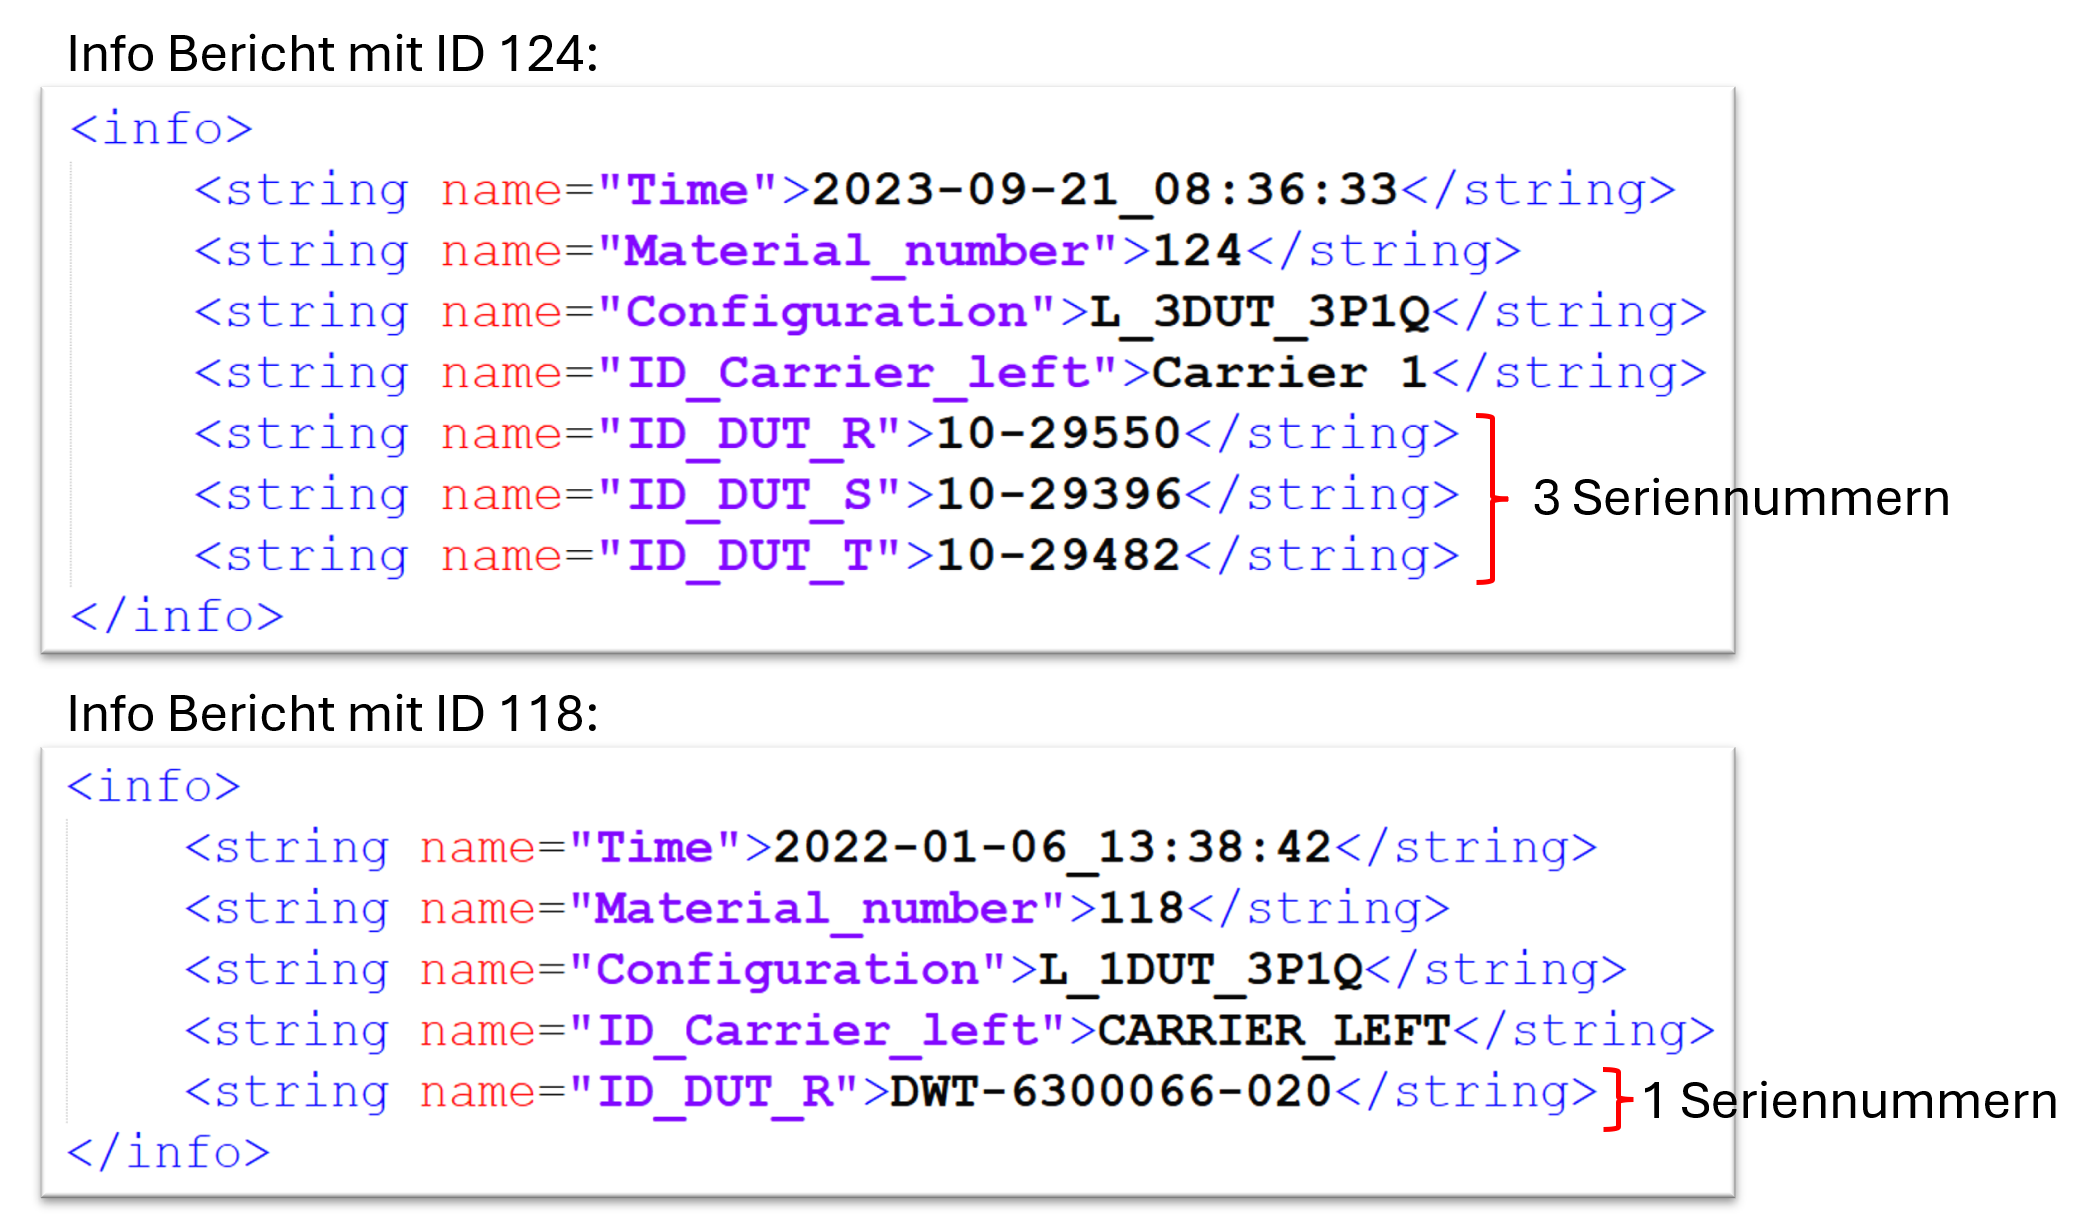
\includegraphics[width=1\textwidth]{Grafiken/Beispiel Fehler Seriennummeranzahl.png}
    \caption{Beispiel Fehler Seriennummeranzahl}
    \label{fig:Beispiel Fehler Seriennummeranzahl}
    {Quelle: Eigene Darstellung}
\end{figure}

\item \textbf{Fehler beim Ausgeben der Flowrate-Graphen} \\
Bei allen gelb markierten Zeilen in der Tabelle \ref{tab: Tabelle der Testergebnisse} fehlte der Graph für die Flowrate der Kühlung.
Dieser Fehler kann auf einen Unterschied in der Benennung des Namens der Messwertreihe zurückgeführt werden.
Die DUTs werden je nach Typ mit Luft oder Wasser gekühlt, wodurch sich der Name der Messwertreihe ändert.
Sie wird zwar richtig in die Datenbank eingelesen, nur die Funktionen für das Suchen und Darstellen kennen nur den Namen für die luftgekühlten DUTs.
Daher muss in diesen Funktionen angepasst werden, um auch die Messwertreihen mit Wasserkühlung zu erfassen und weiterzugeben.
Diese Änderung benötigt keine größeren Anpassungen.
Der Unterschied der XML-Strukturen wird in Abbildung \ref{fig:Beispiel Fehler Wassserkühlung vs Luftkühlung} für eine bessere Veranschaulichung dargestellt.

    \begin{figure}[H]
    \centering
    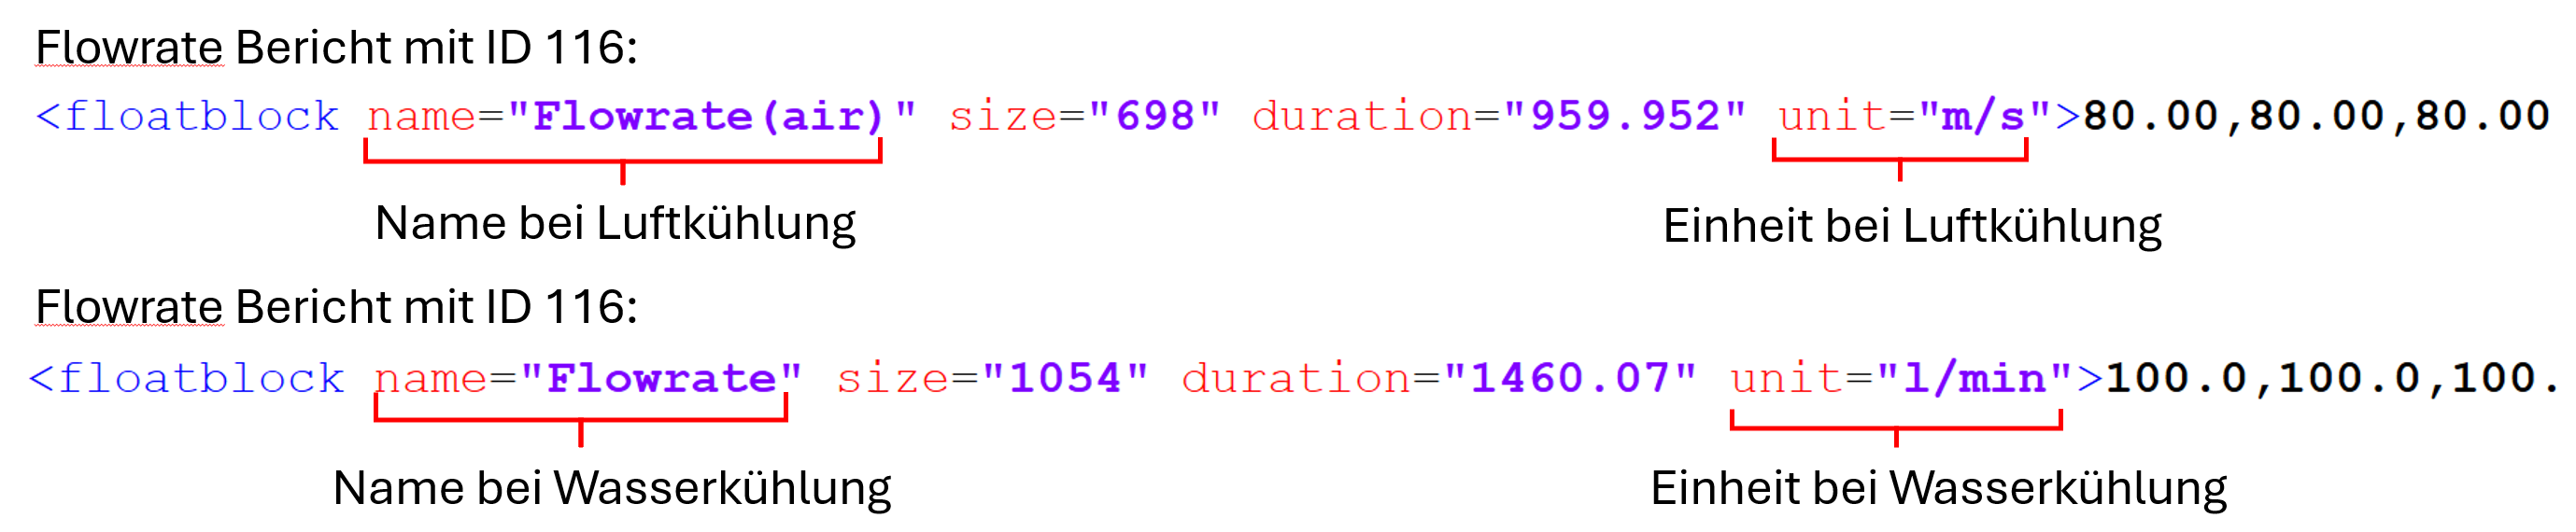
\includegraphics[width=1\textwidth]{Grafiken/Beispiel Fehler Wasserkuehlung vs Luftkuehlung.png}
    \caption{Beispiel Fehler Wassserkühlung vs Luftkühlung}
    \label{fig:Beispiel Fehler Wassserkühlung vs Luftkühlung}
    {Quelle: Eigene Darstellung}

\end{figure}

\end{enumerate}

